\documentclass{article}
\usepackage{fontspec}
\pagestyle{empty}
\usepackage{geometry}
\geometry{paperwidth=50mm, paperheight=40mm, left=2mm, top=0mm, right=2mm, bottom=0mm}
\parindent=0pt
\usepackage{color}
\usepackage{xcolor}
\usepackage{tikz}
\usetikzlibrary{intersections}

\begin{document}
\centering
\vspace*{\fill} \vspace*{-5ex}
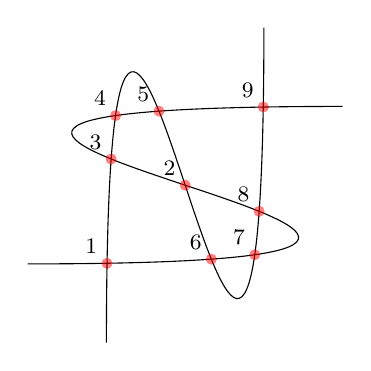
\begin{tikzpicture}
\clip (-2,-2) rectangle (2,2);
\draw [name path=curve 1] (-2,-1) .. controls (8,-1) and (-8,1) .. (2,1);
\draw [name path=curve 2] (-1,-2) .. controls (-1,8) and (1,-8) .. (1,2);
\fill [name intersections={of=curve 1 and curve 2, name=i, total=\t}]
[red, opacity=0.5, every node/.style={above left, black, opacity=1}]
\foreach \s in {1,...,\t}{(i-\s) circle (2pt) node {\footnotesize\s}};
\end{tikzpicture}


\vspace*{\fill} 
\end{document}